\documentclass[10pt]{article} 
\usepackage[final]{graphicx}
\graphicspath{{Fig/}}
\usepackage{epstopdf}
\usepackage{subcaption}
\usepackage{amsfonts} 
\usepackage{url}
\usepackage{amsmath}
\usepackage{tikz, flowchart}
\usepackage{enumitem}
\usepackage[titletoc]{appendix}
\usetikzlibrary{arrows}
\topmargin-.5in 
\textwidth6.6in 
\textheight9in 
\oddsidemargin0in 
 
\def\ds{\displaystyle} 
\def\d{\partial} 

 
\begin{document} 
% PARTICIPANTS, MENTORS, AFFILIATIONS

\centerline{\large \bf Modeling Ebola: Three Distinct Models with Similar Predictions}

\vspace{.1truein}

\def\thefootnote{\arabic{footnote}}
\begin{center}
  Hsuan-Wei Lee\footnote{Department of Mathematics, University of North Carolina Chapel Hill},
  Anzhelika Lyubenko\footnote{Department of Mathematical and Statistical Sciences, University of Colorado Denver},
  Yuhang Ma\footnote{Department of Operations Research and Information Engineering, Cornell University},
  Emily Meissen\footnote{Program of Applied Mathematics, University of Arizona},
  Daniela Velez-Rendon\footnote{Department of Bio-engineering, University of Illinois at Chicago},
    Nara Yoon\footnote{
Department of Mathematics, Applied Mathematics and Statistics, Case Western Reserve University}
\end{center}

%\vspace{.1truein}

\begin{center}
Mentors: John Peach \footnote{Massachusetts Institute of Technology: Lincoln Laboratory}, Cammey Cole Manning\footnote{Mathematics and Computer Science Department, Meredith College},
Christian Gunning\footnote{Departments of Entomology and Mathematics, North Carolina State University}
\end{center}
% ABSTRACT

\begin{abstract}
\noindent We present and compare three models of the Ebola outbreak in Liberia during 2014-2015. We approach the problem from both systematic and agent-based perspectives and compare the results to the actual data as well as between models. We show that if the outbreak is not contained in the early stages and the individuals do not change their behavior as the virus prevails, between 60 and 80 percent of population get the disease. 
\end{abstract}

\tableofcontents

\section{Introduction}
Bacteria growth during wine making, spread of infectious diseases and recruitment to extremists organizations can be modeled in a similar way - either by exponential or logistic growth models. For the purposes of this paper we focus solely on modeling the spread of Ebola through Liberia throughout 2014 - 2015 outbreak. We chose to focus on Liberia because most of the data needed for the model was available in the literature. While the model allows one to consider other countries affected by the outbreak we did not calibrate the associated parameters. 

Ebola was first discovered in 1976. Since then, there were 34 records of Ebola reported by the Center for Disease Control and Prevention. However, until 2014 all outbreaks had a reported number of deaths that did not exceed 500; 11 of them did not exceed 10 individuals and 15 records did not exceed 65 individuals \cite{CDCOutbreaks}.  The outbreak of 2014 is considered different. It took thousands of lives over the past two years and received an extensive media coverage.

The current outbreak may be different because it was the first time Ebola was contracted in the West Africa as opposed to Central Africa where it was first discovered. Early symptoms are flu-like: fever, headache, fatigue and joint pain. Diseases like HIV and Malaria, which are common to the region, have the same symptoms. As Ebola progresses, the infected experiences abdominal pain, diarrhea, vomiting and rashes. The virus is contracted through direct contact with bodily fluids and secretion: blood, saliva, urine, fecal matter. Once virus is contracted, the incubation period may last up to two weeks making intervention measures like tracking difficult \cite{CDCSympt}. 

A variety of cultural and economic factors have contributed to the spread of the disease: lack of medical centers in some regions and poor sensitization practices in such centers, distrust in the western medicine, poverty and traditional burial ceremony which includes physical contact with the diseased \cite{WHOReasons}. 

One may look at the spread of the infectious diseases from two perspectives: system based and agent based. In the system based model the entire population is divided into compartments with a certain proportion of the population in each. As time progresses certain amount of people flow from one compartment into another. Naturally, such relationship is described either by a difference or a differential equation. One of the most well-known equation-based models involves three states: susceptible, infected, recovered. Such model is called an SIR model; each letter in the abbreviation represents one of the compartments in the population. This model has multiple modifications because various compartments can be added. In the case of Ebola, Lekone and Finkenstäd \cite{Lekone2006} consider a four compartment model, inserting an "Exposed" state between "Susceptible" and "Infected". A six-compartment model, presented by Legrand \cite{Legrand2007} and Rivers\cite{Rivers2014} differentiates between the modes of transition of the disease, i.e. a virus can be transmitted in the community, at hospitals and medical centers or at funerals.

In contrast to system based models, agent-based models are concerned with the behavior of a typical individual rather than the system as a whole. In such models every individual in the system is assigned certain characteristics, i.e. states. Individual's behavior is probabilistic at each unit of time and causes him either to transition to a different state or stay in his current state. Agent-based models for Ebola include Siettos et al. \cite{Siettos2015} and Merler et al.\cite{Merler2015}. A variety of models examine the effectiveness of intervention measures. Examples include contact tracing by Webb et al. \cite{Webb2015} and travel restrictions by Poletto et al. \cite{Poletto2014}.

In this paper we consider a seven-compartment model, both system and agent-based. We show \textbf{What did we show?!} \textbf{What about the model with spatial component?}

In section~\ref{sec:Model} we present our model. Section~\ref{sec:Data} describes our data and parameters. Section~\ref{sec:Results} discusses the results of numerical experiments. Section~\ref{sec:Summary} concludes.

It should be written as much as possible in non-technical terms, so that a
lay reader can understand the context and the contribution of the paper.

\begin{itemize}
\item Describe the problem you are trying to solve, the approach
you took, and summarize your contribution and results.

\item Review the history of this problem, and existing literature.

\item Give an outline of the rest of the paper.
\end{itemize}


\section{Methods}
We examine the problem from two perspectives. We present a system based model first and then discuss an agent-based modification of it. We then consider an agent-based model that incorporates agents' movement through space. Throughout the three models we utilize the same assumptions and compartment-state definitions. 

In order to propose a more accurate model and compare the results among different programming  languages, the compartment flow model of the Ebola Epidemic in West Africa, 2014, was modeled with a System Dynamics (SD) and Agent Based Model (ABM) approaches.  Insight Maker and Mathematica was utilized  for the SD, and Insight Maker and Python for the ABM.\\

\begin{itemize}
\item We consider a model of Ebola Outbreak with parameters calibrated for Liberia.
\item We consider two time periods. The first one starts with the announcement of Ebola outbreak in March 2014 and ends the day of the International Intervention in September 2014. The second period covers the time from the International Intervention to July 2015.
\item We ignore all the possible births and deaths occurred due to reasons other that Ebola during the chosen time. 
\item Each individual who dies because of Ebola has a funeral.
\end{itemize}



\subsection{Compartment-State Definition}
Based on the compartmental model and parameters published by Rivers et al.\cite{Rivers2014} in October 2014, it was modeled a similar approach.  This particular model, divides the population into six different compartments; the Susceptible persons (S) could become Exposed (E), if they were in contact with an infected individual, initiating a transition to the Infectious (I) state after the incubation period of the disease, subsequently, acquiring the capacity of infecting others. A percentage of the I class individuals may be Hospitalized (H). There are two possible outcomes for the untreated individuals in I and the treated patients in H, individuals may die, with a probability of infecting other people during the resultant Funeral (F), before the virus is removed (R) from the individual, or the patients may recover, at this stage, can be considered equivalently removed. However,  in order to distinguish between the recovered (R) patients and the deceased (D) individuals, was considered a model with seven compartments : S, E, I, H, F, R and D. Figure ~\ref{fig:compartmentNoFlow} depicts the implemented compartment model. \\


\begin{figure}[!h]
  \centering
  \includegraphics[width=1\textwidth]{compartmentNoFlow}
  \caption{Compartment Model of the Ebola Epidemic in Liberia. \newline  Being S: Susceptible, E: Exposed, I: Infectious, H: Hospitalized, F: Funeral,  R: Recovered and D: Dead.  } 
\label{fig:compartmentNoFlow} 
\end{figure}

\begin{description}
\item[S]- Susceptible. Individuals who have not contracted the disease and have no immunity to it. 
\item[E] - Exposed. Individuals who have come in contact with the Ebola patient and have contracted the disease but do not yet exhibit severe symptoms and thus, are considered not infectious.
\item[I] - Infected. Individuals who experience severe symptoms of Ebola and are contagious.
\item[H] - Hospitalized. Individuals who are infectious and are in the hospital because they are experiencing severe symptoms of Ebola.
\item[F] - Funeral. Diseased but still contagious victims of Ebola. 
\item[D] - Dead. Individuals who died because of Ebola and have been buried. They are considered not to be contagious.
\item[R] - Recovered. Individuals who had Ebola, survived and now are immune to the disease.
\end{description}


 
The governing equations of the system dynamics described above are the following:
\begin{eqnarray} 
\label{SDeqn}
\frac{dS}{dt} = - \frac{\beta_{I}SI+\beta_{H}SH+\beta_{F}SF}{N}\\
\frac{dE}{dt} =  \frac{\beta_{I}SI+\beta_{H}SH+\beta_{F}SF}{N}-\alpha E\\
\frac{dI}{dt} =  \alpha E - [\gamma_{H}\theta + \gamma_{I}(1-\theta)(1-\delta_{1})+\gamma_{D}(1-\theta)\delta_{1}]I\\
\frac{dH}{dt} = \gamma_{H}\theta I - [\gamma_{DH}\delta_{2}+\gamma_{IH}(1-\delta_{2})]H\\
\frac{dF}{dt} = \gamma_{D}(1-\theta) \delta_{1} I + \gamma_{DH}\delta_{2} H-\gamma_{F} F\\
\frac{dR}{dt} = \gamma_{I}(1-\theta)(1- \delta_{1}) I + \gamma_{IH}(1-\delta_{2}) H-\gamma_{F} F
\end{eqnarray}
where each of the parameters are defined on Table \ref{tab:parameters}






%\section{System Dynamics}
% Insight Maker is a powerful online tool used to model and simulate complex systems. It utilizes different approaches, such as System Dynamics, Agent-Based Modeling and imperative programming. Insight Makera construction of a graphical model to forecast the system response \cite{FortmannRoe}. We used the InsightMaker platform to prototype our model and simulate stepping forward through time. More details about the platform and its functionality can be found in Fortmann-Roe's review \cite{FortmannRoe}. The platform uses a fourth order Runge-Kutta differential equation solver for the system dynamics model and  first order Euler approximation for the Agent-Based model.

\noindent A normalized population fraction was simulated. The compartment S was initialized with a value of 999.999/1.000.000, and the compartment I with 1/1.000.000, meaning that there is an infected individual per every million of individuals, the rest of the compartments were set to zero as an initial condition. The flow between the compartments is specified in Figure \ref{fig:compartment.} and all the other parameters were initialized as shown in Table \ref{tab:parameters}.  As mention in Section \ref{sec:calibration}, the parameters were calibrated in two stages, before and after the international intervention. According with the time frame proposed, the change in the parameters was also implemented on Insight Maker. The links to the online models can be found on \cite{IM_AI} and  \cite{IM_BI}.  


% RESULTS AND DISCUSSION
%
%No intervention
\noindent After modeling the system with the parameters before the intervention, it can be observed in Figure \ref{fig:LB_IM_NoIn} how the total population decreases to 46.46\%  if there is no intervention and the each of the parameters continue to be the same. The number of susceptible individuals exponentially decays, converging to 7\% of the population, while exposed, infected, hospitalized and funeral comparments converges to zero; finally, after the system stabilizes, the final proportion of deaths would be 53.53\% 

\begin{figure}[!h]
  \centering
  \includegraphics[width=1\textwidth]{LB_NoInt_SD_IM}
  \caption{ Insight Maker results using the parameters of the first stage (Mar/14 to Sept/14) and assuming no intervention}
\label{fig:LB_IM_NoIn} 
\end{figure}

%Intervention 
\noindent As mentioned before, five parameters were calibrated for the second stage of the Ebola Outbreak, namely, community contact rate ($\beta_I$), hospital contact rate ($\beta_H$), funeral contact rate ($\beta_F$), time until hospitalization ($\gamma_H$) and probability a case is hospitalized ($\theta$). Figure \ref{fig:LB_IM_In} A. shows that there is not much change in the Total population and susceptible compartment, meaning that the virus was controlled;  Figure \ref{fig:LB_IM_In} B focuses on E, I, R, H , F and D compartments, showing that the international intervention causes a dramatic change in the behavior of such compartments.

\begin{figure}[!h]
  \centering
  \includegraphics[width=1\textwidth]{LB_Int3_SD_IM}
  \caption{ Insight Maker results. \textit{A.} Parameters of the first stage (Mar/14 to Sept/14), \textit{B.} Parameters of the second stage ( Sept/14 to July/15)}
\label{fig:LB_IM_In} 
\end{figure}


%Comparing with WHO data

\noindent Finally, a comparison between the proposed model and World Health Organization data is shown in Figures \ref{fig:LB_IM_WHO} and \ref{fig:LB_IM_WHO2}. As depicted in Figure \ref{fig:LB_IM_WHO} A and B there is a good fitting of our model with the data reported by WHO. Figure \ref{fig:LB_IM_WHO2} shows  the reported WHO data before and after intervention, the results of our model before and after intervention and the forecast for the coming months, predicting that after the system reaches an equilibrium, the proportion of deaths in Liberia product of the EVD would be 5.07\% approximately.


\begin{figure}[!h]
  \centering
  \includegraphics[width=1\textwidth]{LB_BI_AI_SD_WHO_IM}
  \caption{ Comparison between World Health Organization (WHO) data and Insight Maker (IM) results using the parameters of A. the first stage (Mar/14 to Sept/14) and B. the second stage ( Sept/14 to July/15) for the cumulative deaths (D).}
\label{fig:LB_IM_WHO} 
\end{figure}



\begin{figure}[!h]
  \centering
  \includegraphics[width=1\textwidth]{LB_Int2_SD_WHO_IM}
  \caption{ Comparison between World Health Organization (WHO) data and Insight Maker (IM) results using the parameters before intervention (BI) and after intervention (AI), for the cumulative deaths (D).}
\label{fig:LB_IM_WHO2} 
\end{figure}


%%MATHEMATICA DESCRIPTION
\newpage
\subsection{Mathematica}
We drew the plots in the previous section also with Mathematica, and got almost same result. One additional plot we draw in Mathematica is phase portrait of the system (Figure).

\begin{figure}[!h]
  \centering
  \includegraphics[width=1\textwidth]{PhasePortrait}
  \caption{Projection of phase portrait to (Susceptible + Recovered, Dead) space. (Blue) - without intervention, (Red) - with intervention, (Dots) - where the phase converges (equilibrium).}
\label{fig:Phase Portrait}
\end{figure}
 %includes parameter calibration, insight maker and mathematica results
%

%\section{Agent-Based Dynamics}
%The next model we consider is an agent-based model. Each individual in the population can be in one of 7 states discussed above: susceptible, exposed, infected, hospitalized, funeral, recovered or dead. The flow between two states is a  probability of transition from one state to another for a typical individual. We represent our model in Figure~\ref{ABM}. In each time step a typical individual who is susceptible to contracting a virus can either transition to an exposed state with probability $p_{SE}$ or stay susceptible with probability $p_{SS}$. An individual in the exposed state transitions to infected with probability $p_{EI}$ and stays exposed with probability $p_{EE}$. An individual who is infected can stay infected, recover, go to a hospital or die and transition to funeral state with probabilities $p_{II},\, p_{IR},\, p_{IH}$ and $p_{IF}$ respectively. Recovery is considered a terminal state so individuals in this state stay in it for the remaining duration of the simulation. Hospitalized individuals may stay hospitalized, transition to recovered or funeral with probabilities $p_{HH}, \, p_{HR}$ and $p_{HF}$. We assume that the individual who dies from Ebola remains infectious through the duration of the entire burial ceremony and no precautions are taken against disease transmission. Safely buried individuals are considered noninfectious and remain in this state for the remaining time of the simulation.  

%  \begin{tikzpicture}[node distance=2cm, font=\tiny]
%        \node [draw, terminal]  (start) at (0,0) {Start};
%        \node [draw, predproc, right of= start] (acquire)(write) {Acquire Image};
%
%%% paths
%    \draw[->](work) -- node[above]{yes}(end);
%    \end{tikzpicture}
\begin{figure}[h!]
\begin{center}
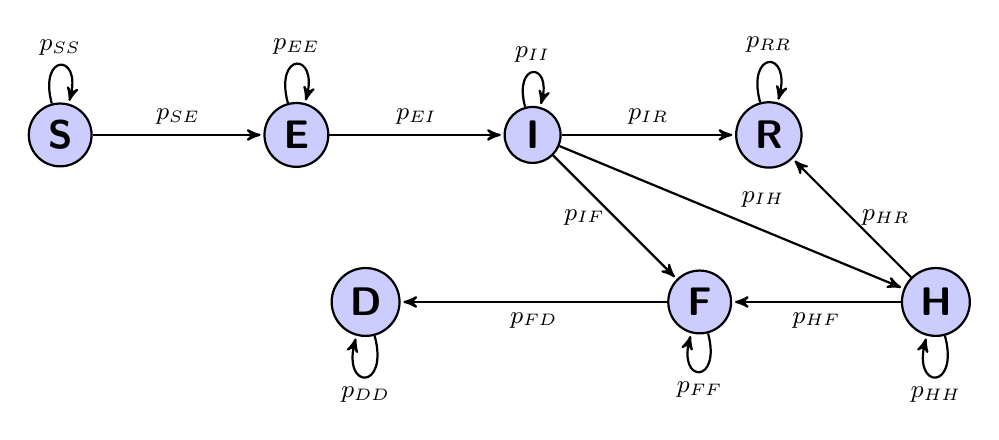
\begin{tikzpicture}[->,>=stealth',shorten >=1pt,auto,node distance=3cm,
  thick,main node/.style={circle,fill=blue!20,draw,font=\sffamily\Large\bfseries}]

  \node[main node] (1) {S};
  \node[main node] (2) [right of=1] {E};
  \node[main node] (3) [right of=2] {I};
  \node[main node] (4) [right of=3] {R};
    \node[main node] (5) [below left of=3] {D};
      \node[main node] (6) [below right of=3] {F};
        \node[main node] (7) [right of=6] {H};

  \path[every node/.style={font=\sffamily\small}]
    (1)
        edge node {$p_{SE}$} (2)
        edge [loop above] node {$p_{SS}$} (1)
    (2) 
        edge node {$p_{EI}$} (3)
         edge [loop above] node {$p_{EE}$} (2)
      
    (3) 
       edge node {$p_{IR}$} (4)
       edge node[left] {$p_{IF}$} (6)
       edge node {$p_{IH}$} (7)
        edge [loop above] node {$p_{II}$} (3)
    (4)
         edge [loop above] node {$p_{RR}$} (4)
       
(6) edge node{$p_{FD}$} (5) 
edge [loop below] node {$p_{FF}$} (6)     
(7) edge node[right]{$p_{HR}$} (4) 
edge [loop below] node {$p_{HH}$} (7)
  (7) edge node{$p_{HF}$} (6)      
 (5) edge [loop below] node {$p_{DD}$} (5)
        ;
        
\end{tikzpicture}
\end{center}
\caption{Spread of the disease: Agent-based model. Each node represents a typical individual's state. An individual can transition to a state to which he is connected by a directed arc with a probability specified on an arc.}
\label{ABM}
\end{figure}
Let

\begin{itemize}
\item[] $N$  total number of individuals in a population
\item[] $N_{I}$  total number of individuals in the infected state
\item[] $N_{H}$  total number of individuals in the hospitalized state
\item[] $N_{F}$  total number of individuals in the funeral state
\end{itemize}
We define and present numeric values of individual's probability of transition for each state in Table~\ref{tab:probabilities}. In calculating the probabilities we used data from Table~\ref{tab:knownParameters} and Table~\ref{tab:calibratedParameters}

\begin{table}[h!]
\caption{Agent-based Model Parameters for Ebola Epidemic in Liberia Before and After the International Intervention} % title of Table
\centering % used for centering table
\begin{tabular}{c c c c} 
\hline\hline %inserts double horizontal lines
Parameter & Definition&  Liberia Before Intervention  & Liberia After Intervention \\ %[0.5ex] 
& & (Mar 2014 to Sept 2014) &  (Sept 2014 to Jul 2015) \\ %[0.5ex] % inserts table
% inserts table
%heading
\hline % inserts single horizontal line
$p_{SE}$	 &$\beta_I N_{I}/N+\beta_H N_{H}/N+\beta_F  N_F/ N$ 	& \textbf{Dynamic}	 & \textbf{Dynamic} \\ 
$p_{SS}$ 	& $1-p_{SE}$													 & \textbf{Dynamic}	 & \textbf{Dynamic}  \\ 
$p_{EE}$ 	& $1-1/t_{P}$ 												& 0.9091 			& 0.9091  \\ 
$p_{EI}$ 	& $1/t_{P}$ 												&0.0909			 & 0.0909  \\ 
$p_{II}$ 	& $1/t_{I}$ 												& 0.1 				& 0.1  \\ 
$p_{IH}$	 & $1/t_{H}$ 												&0.2227 			& 0.2160  \\ 
$p_{IF}$ 	& $1/t_{D}$ 												& 0.125 			& 0.125  \\ 
$p_{IR}$ 	& $1-p_{II}-p_{IH}-p_{IF}$ 											&0.5523 			& 0.559  \\ 
$p_{HF}$ 	& $1/t_{DH}$												& 0.2849 			& 0.2849 \\ 
$p_{HR}$ 	& $1/t_{IH}$ 												&0.1815 			& 0.1815 \\ 
$p_{HH}$ 	& $1-p_{HF}-p_{HR}$ 												& 0.5336			& 0.5336  \\ 
$p_{FF}$ 	& $1/t_{F}$ 												&  0.5 			& 0.5 \\ 
$p_{FD}$ 	& $1-p_{FF}$													 & 0.5 			& 0.5  \\ 
$p_{RR}$ 	& 1															& 1 				& 1  \\ 
$p_{DD}$ 	& 1															&1				 & 1 \\ [1ex] 
\hline 
\end{tabular}
\label{tab:probabilities}
\end{table}
\subsection{Simulation}
We consider a population of size 1000 with 999 individuals starting in a susceptible state and 1 individual in the exposed state. Numeric probabilities of an individual transitioning from each state are recorded in Table~\ref{tab:probabilities}. We run a hundred Monte Carlo simulations and average the results to estimate an outcome of the disease. We define an outbreak as an event in which 1\% of the population or more contracts the disease. If only one individual is exposed to the disease in a population of 1000, there is about 30\% chance that the outbreak does not happen (27/100 cases). However, once the cumulative proportion of the exposed individuals reaches 1\%, the virus affects more than 90\% of the population. A histogram for simulation outcomes is depicted in Figure~\ref{fig:Hist}.
%
%
% HERE IS THE PROBABILITY TRANSITION TABLE
%
%
%
%
\textbf{TALK ABOUT THE COMPLICATED EQUATION}
\begin{figure}
\begin{center}
\includegraphics[scale=0.5]{N1000Hist.eps}
\end{center}
\caption{Histogram showing the outcome of 100 simulations.}
\label{fig:Hist}
\end{figure}


%%%%%%%%%%%%%%%%%%%%%%%%%%%%%%%%%%%%
% figure N1000Hist.eps
%%%%%%%%%%%%%%%%%%%%%%%%%%%%%%%%%%%%
We note that the simulations reach their stationary state before $t = 500$. We plot the result of 100 simulations in Figure~\ref{fig:Scatter}. In many cases we don't observe an outbreak of Ebola. However there are many cases which show catastrophic disease. In the disastrous case, on average, 95\% of people get the disease and 76\% of people die from it. 

%%%%%%%%%%%%%%%%%%%%%%%%%%%%%%%%%%%%
% figure N1000Scatter.eps
%%%%%%%%%%%%%%%%%%%%%%%%%%%%%%%%%%%%
 
\begin{figure}
\begin{center}
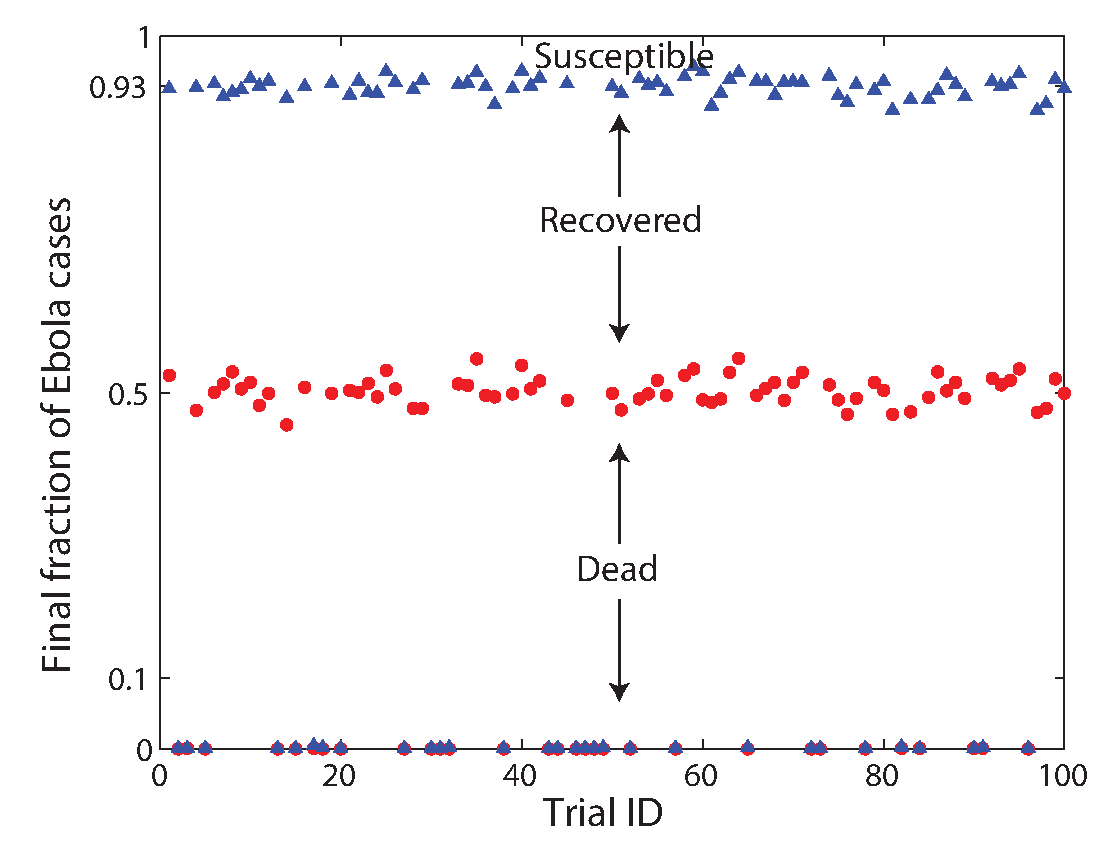
\includegraphics[scale=0.5]{N1000Scatter.eps}
\end{center}
\caption{Scatter plot showing the proportion of population that contracts the disease and the proportion of the population that dies due to the disease for a population size 1000}
\label{fig:Scatter}
\end{figure}

%%%%%%%%%%%%%%%%%%%%%%%%%%%%%%%%%%%%
% figure N1000Scatter.eps
%%%%%%%%%%%%%%%%%%%%%%%%%%%%%%%%%%%%

If there is no outbreak, the infected agent may or may not infect another agent in the population. However, most people remain in the  susceptible state because the infected individual recovers or dies before he infects enough people to cause an outbreak. The proportion of the population that gets Ebola is low, so all seven states stay relatively constant over time. %Illustration of this case is presented in Figure~\ref{fig:NoOutbreak}.
%\begin{figure}
%\begin{center}
%\includegraphics[scale=0.8]{NoOutbreak.eps}
%\end{center}
%\caption{No outbreak realization of the outbreak process}
%\label{fig:NoOutbreak}
%\end{figure}

%%%%%%%%%%%%%%%%%%%%%%%%%%%%%%%%%%%%
% figure NoOutbreak.eps
%%%%%%%%%%%%%%%%%%%%%%%%%%%%%%%%%%%%

On the other hand, if the infected agent contacts many people during the time he is infected (I), hospitalized (H), or in a funeral state (F) before he transitions to state D or R, there is a an outbreak of the disease. A typical outbreak is depicted in Figure~\ref{fig:Outbreak}. The proportion of agents who contract the disease grows exponentially until $t = 125$. That is also the time at which the proportion of population  in states I, H, and F is the highest. After that, the population does not have enough susceptible agents to spread the disease causing the proportion of exposed agents to decrease. The proportion of agents in I, H, and F decreases as well. Around $t = 180$ the proportion of the population is states I, H, and F is zero; the proportion of the population in state S does not decrease, i.e. no agents get Ebola. At this point, every agent remains in S, R or D and an equilibrium is reached (stable fixed point). As we showed before, on average, 5\% of agents stay in state S, 19\% of agents stay in R, and 76\% of agents would be in D. 
%%%%%%%%%%%%%%%%%%%%%%%%%%%%%%%%%%%%
% figure Outbreak.eps
%%%%%%%%%%%%%%%%%%%%%%%%%%%%%%%%%%%%
\begin{figure}
\begin{center}
\includegraphics[scale=0.8]{Outbreak.eps}
\end{center}
\caption{Realization in which outbreak occurs}
\label{fig:Outbreak}
\end{figure}

%%%%%%%%%%%%%%%%%%%%%%%%%%%%%%%%%%%%
% figure Outbreak.eps
%%%%%%%%%%%%%%%%%%%%%%%%%%%%%%%%%%%%


\textbf{Choose how you want to word it; Maybe move description to caption of the figure. Also need to cite only once. Either at the beginning or later}.
We plot a phase portrait for the proportion of agents who never got infected and are in S vs. the proportion of agents who contracted the disease (both D and R) as time progresses.The result is presented in Figure~\ref{fig:PhasePortraitABM}. On the horizontal axis, we put the ratio of S to the total population and on the vertical axis - the ratio of D plus R to the total population.  When $t = 0$, one agent is in state E and 99.9\% of agents are in S. All other states contain no agents. About 30\% of the time, there is no severe outbreak. In such case, only few people get Ebola. As time goes by there are only few transitions between states and a stationary point is reached within a few time steps. However, if there is an outbreak, the trajectory gradually moves to its equilibrium state. On average, the equilibrium occurs at $(S, R+ D) = (0.05, 0.95)$. We conduct ten experiments and plot their trajectories on the same graph, presented in Figure~\ref{fig:PhasePortraitABM}. Because the total proportion of people in the population is one, the equilibria in different experiments lie on the $x + y = 1$ line. The system starts at $(S, [R]+[D]) = (0.999, 0)$, a point that is close to this line. During the course of the outbreak, the phase portrait falls below the x + y = 1 line because a portion of the population are in the transient states: E, I, H and F. 

%%%%%%%%%%%%%%%%%%%%%%%%%%%%%%%%%%%%
% figure PhasePortrait.eps
%%%%%%%%%%%%%%%%%%%%%%%%%%%%%%%%%%%%
\begin{figure}[h!]
\begin{center}
\includegraphics[scale=0.5]{PhasePortrait.eps}
\end{center}
\caption{Phase portrait: proportion of the population who are in susceptible state vs. population of the population who contracted Ebola for different uncertainty realizations.}
\label{fig:PhasePortraitABM}
\end{figure}

%%%%%%%%%%%%%%%%%%%%%%%%%%%%%%%%%%%%
% figure PhasePortrait.eps
%%%%%%%%%%%%%%%%%%%%%%%%%%%%%%%%%%%%

As in the Systems Dynamics approach, we perform an intervention in the agent-based model. Because the scale in the two models is different, we implement the intervention step if we see an outbreak, i.e. when 1\% of agents are in state E. At the beginning of intervention, we change the three $\beta$s, representing the different contact rates. Our results, presented in Figure~\ref{fig:Intervention}, show that if we start the intervention at 1\% of population having Ebola, 4\% of agents get the disease, 1\% of agents recover and 3\% of agents die. This is a significant improvement over the disastrous predicted outcome of an outbreak without an intervention. 

%%%%%%%%%%%%%%%%%%%%%%%%%%%%%%%%%%%%
% figure InterventionZoomIn.eps
%%%%%%%%%%%%%%%%%%%%%%%%%%%%%%%%%%%%

\begin{figure}[h!]
\begin{center}
\includegraphics[scale=0.8]{InterventionZoomIn.eps}
\end{center}
\caption{Effect of Intervention on the spread of the disease }
\label{fig:Intervention}
\end{figure}

%%%%%%%%%%%%%%%%%%%%%%%%%%%%%%%%%%%%
% figure InterventionZoomIn.eps
%%%%%%%%%%%%%%%%%%%%%%%%%%%%%%%%%%%%

We examine the effect of the population size on the outcome of the agent-based model. Besides the baseline case of $N = 1000$, we set the total population to be $N = 100$ and $5000$. The results, presented in Figure~\ref{fig:VarPopSize}, show that an increase in population size decreases the standard deviation of the quantities S, D and R, but the relative averages remain the same. The standard deviation of the number of agents with Ebola becomes smaller as population size increases. This suggests that the system becomes more stable. An important implication of this result is that the predicted outcome is more reliable for larger systems.


\begin{figure} 
\centering 
\begin{subfigure}[b]{0.3\textwidth} \includegraphics[scale=.35]{N100Scatter.eps} \caption{Scatter plot showing the proportion of population that contracts the disease (blue) and dies (red) for a population size 100} \label{fig:N100} \end{subfigure} 
\hfill 
 \begin{subfigure}[b]{0.3\textwidth} \includegraphics[scale=0.35]{N5000Scatter.eps} \caption{Scatter plot showing the proportion of population that contracts the disease (blue) and dies (red) for a population size 5000} \label{fig:N5000} \end{subfigure} 
 \caption{Effect of changing the population size on the proportion of the diseased population}\label{fig:VarPopSize}
  \end{figure}

%%%%%%%%%%%%%%%%%%%%%%%%%%%%%%%%%%%%
%%%%%%%%%%%%%%%%%%%%%%%%%%%%%%%%%%%%
%%%%%%%%%%%%%%%%%%%%%%%%%%%%%%%%%%%%












\section{Spatial Agent-Based Dyanmics}

We next look at an agent-based model where agents are allowed to move within and between cities. Incorporating spatial movement requires making additional assumptions about the map on which movement is allowed and the movement of individuals. The model is coded in \texttt{Python} and propagates the infection and spatial information in discrete days. 

\subsection{Spatial Assumptions}
We restrict the space (on which cities and individuals are located) to a specified width and height and generate cities randomly within the space with specified variance and relative density. For example, a model may have one city with variance $30$ and density $0.9$ and a village with variance $5$ and density $0.1$. Locations of individuals and cities are real numbers stored as \texttt{floats}. We also create a grid, which partitions the individuals based on their location and is used to determine the closest neighbors for community infection and funeral attendance. A family is assumed to have $n_{fam}$ members all of which live in the same exact location. Upon initialization (and later travel), families are place based on the specified city densities, normally distributed around the city's center location using the city's variance. We define an individual's \emph{home} as their initial location.

An individual is \emph{movable} if he is susceptible, exposed, or recovered. All other individuals remain stationary. Movable individuals travel each timestep with probability $p_{trav}$. If they are away from home, they will travel home with probability $p_{home}$. Otherwise, they will travel locally (within their current city or village) or non-locally (to another city) based on the density of their current city. It is assumed that when an individual is in a density with higher density they are less likely to leave. If individual $i$'s current city density (percentage of the total population) is $d[i]$, then the non-local travel probability is $(1-d[i])/2$. In the local and non-local travel, the individual is again normally distributed around that city's center.

\subsection{Agent Behavior}
\begin{figure}[h!t]
\begin{center}
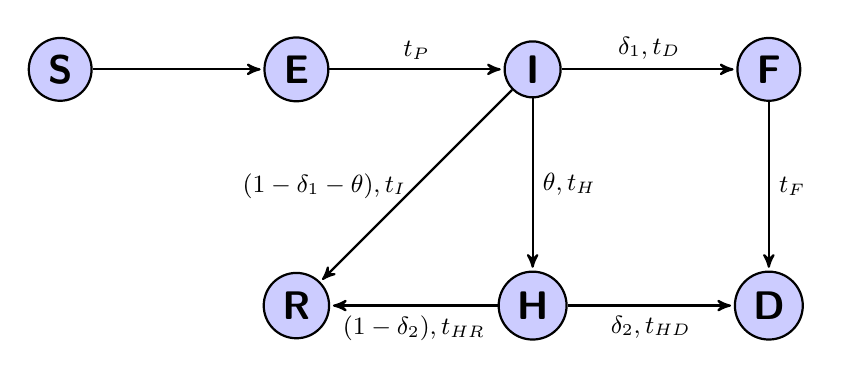
\begin{tikzpicture}[->,>=stealth',shorten >=1pt,auto,node distance=3cm,
  thick,main node/.style={circle,fill=blue!20,draw,font=\sffamily\Large\bfseries}]

  \node[main node] (1) {S};
  \node[main node] (2) [right of=1] {E};
  \node[main node] (3) [right of=2] {I};
  \node[main node] (4) [right of=3] {F};
  \node[main node] (5) [below of=3] {H};
  \node[main node] (6) [below of=4] {D};
  \node[main node] (7) [left of=5] {R};

  \path[every node/.style={font=\sffamily\small}]
    (1)
        edge node {$ $} (2)
        %edge [loop above] node {$1-p_{SE}$} (1)
    (2) 
        edge node {$t_P$} (3)
        % edge [loop above] node {} (2)
      
    (3) 
       edge node {$\delta_1, t_D$} (4)
       edge node[right] {$\theta, t_H$} (5)
       edge node[left] {$(1-\delta_1-\theta), t_I$} (7)
        %edge [loop above] node {$p_{II}$} (3)
    (4)
         edge node {$t_F$} (6)
        % edge [loop above] node {$p_{FD}$} (6)
       
(5) edge node[below] {$\delta_2, t_{HD}$} (6) 
	edge node {$(1-\delta_2), t_{HR}$} (7)
%edge [loop below] node {$p_{FF}$} (6)     
;
        
\end{tikzpicture}
\end{center}
\caption{Available states for individuals and the transitions between them. Probabilistic transitions and timeouts between states are listed along the transitions. If both are present, once it is decided that the individual will transition, the timeout is calculated and counted down. The transition from susceptible to exposed is based on the surrounding infected individuals using transmission probabilities $\eta_f,\eta_c,\eta_F$.}
\label{fig:sabm-states}
\end{figure}

The model uses the same states as the previous models, but some of the transitions and probabilities have been modified. Specifically, hospitalized individuals are assumed to be quarantined, and thus no longer infect others or have funerals. Instead, hospitalized individuals move straight to the dead state upon death. See Figure \ref{ABM} vs Figure \ref{fig:sabm-states} for a comparison between the two agent-based models. Figure \ref{fig:sabm-states} denotes the probabilistic and timeout transitions between states. We define a \emph{timeout} to be an integer number of days to wait before transitioning to another state, either uniformly randomly generated between two in or equal to a specified constant. Whenever a range of integers is listed, the integer used in simulation is uniformly drawn from that range.

The spatial movement and transitions between states is dependent on the individual's current state. Following are a description of the behavior of each type of individual.
\begin{description}[labelsep=1.5mm]
\setlength\itemsep{-3mm}
\item[Susceptible] individuals travel randomly and may only transition to the exposed state.\\
\item[Exposed] individuals may also travel randomly. Upon initial transition, they generate a timeout of $t_P$ days until they will transition to the infected state.\\
\item[Infected] individuals are assumed to be too sick to travel. Upon initial transition, it is decided whether they will go to the hospital (with probability $\theta$, generating a timeout of $t_H$ until transitioning to hospitalization), die and be buried at a funeral (with probability $\delta_1$, generating a timeout of $t_D$ until transitioning to the funeralized state), or recover (generating a timeout of $t_I$ until transitioning to the recovered state). While in the infected state, the individual infects people in the surrounding grid each with probability $\eta_f$ if they are a family member or $\eta_c$ otherwise. See Figure \ref{fig:infect} for a visualization.\\
\item[Hospitalized] individuals are quarantined and no longer infect anyone. Upon initial transition, it is decided whether they will die in the hospital (with probability $\delta_2$, generating a timeout of $t_{HD}$ until death) or recover (generating a timeout of $t_{HR}$ until recovery). Because they are quarantined, traditional funerals with high infection rates are not held upon death.\\
\item[Funeralized] individuals spend $t_F$ days in the funeralized state before transitioning to the dead state, but only infect people on the initial entrance to the funeralized state. Upon initial transition, the individual and all of his movable relatives return home. All susceptible people in his home grid cell who were also in that grid cell at initialization (family and initial neighbors not currently away) are then infected with probability $\eta_F$. See Figure \ref{fig:infect}.\\
\item[Recovered] individuals do not affect the model but can continue traveling.\\
\item[Dead] individuals remain stationary and do not affect the model.\\
\end{description}

\begin{figure}[h!]
\begin{center}
\begin{tikzpicture}[scale=.6]
\draw [fill=red] (0,0) rectangle (3,3);
\draw[pattern=north west lines, pattern color=black] (1,1) rectangle (2,2);
\draw[step=1cm, thin] (-2,-2) grid (5,5);
\draw[fill=black] (1.7,1.2) circle (.05cm);

\draw[pattern=north west lines, pattern color=black] (6,4) rectangle (6.5,4.5);
\node[anchor=west] at (7,4.25) {funeral};
\draw[fill=red] (6,3) rectangle (6.5,3.5);
\node[anchor=west] at (7,3.25) {community};
\end{tikzpicture}
\end{center}
\caption{Grid cells affected by funeral and community infection. Family infection occurs in the same region as community infection during the normal infection process or in the same region as funeral infection during the funeral infection process.}
\label{fig:infect}
\end{figure}

\subsection{Parameters}

%\begin{table}[ht]
%\caption{Model Parameters for Ebola Epidemic in Liberia Before  and After the International Intervention} % title of Table
%\centering % used for centering table
%\begin{tabular}{c c c } 
%\hline\hline %inserts double horizontal lines
%Parameter & Liberia Before Intervention  & Liberia After Intervention \\ [0.5ex] 
% & (Mar/14 to Sept/14) &  (Sept/14 to Jul/15) \\ [0.5ex] % inserts table
%% inserts table
%%heading
%\hline % inserts single horizontal line
%Contact Rate, Community  ($\beta_{I}$) & 0.148 & 0.0446  \\ 
%Contact Rate, Hospital  ($\beta_{H}$) & 0.235 & 0.0877  \\
%Contact Rate, Funeral  ($\beta_{F}$) & 0.465 & 0.283 \\
%Incubation Period (${1}/{\alpha}$) & 11 days & 11 days  \\
%Time until Hospitalization (${1}/{\gamma_{H}}$) & 4.49 days & 4.63 days  \\
%Time from Hospitalization to Death (${1}/{\gamma_{DH}}$) & 3.51 days & 3.51 days  \\ 
%Duration of Traditional Funeral (${1}/{\gamma_{F}}$) & 2.00 days & 2.00 days  \\
%Duration of Infection (${1}/{\gamma_{I}}$) & 10.00 days & 10.00 days  \\
%Time from Infection to Death (${1}/{\gamma_{D}}$) & 8.00 days & 8.00 days  \\
%Time from Hospitalization to Recovery (${1}/{\gamma_{IH}}$) & 5.51 days & 5.51 days  \\
%Probability a Case is Hospitalized ($\theta$) & 0.248 & 0.233 \\
%Case Fatality Rate, Unhospitalized ($\delta_{1}$) & 0.500  & 0.500  \\
%Case Fatality Rate, Hospitalized ($\delta_{2}$) & 0.500 & 0.500 \\ [1ex] 
%\hline 
%\end{tabular}
%\label{tab:parameters}
%\end{table}


\begin{table}[!Hht]
\begin{center}
\begin{tabular}{c c c}\hline\hline
Parameter & Variable & Value\\\hline\hline
Travel probability & $p_{trav}$ & 0.2\\
Travel, home probability & $p_{home}$ & 0.5\\
Travel, non-locally probability & $p_{nonloc}$ & $(1-\text{current city density})/2$\\
Family size & $n_{fam}$ & 3-6\\\hline
Family infection probability per day & $\eta_f$ & 0.1\\
Community infection probability per day & $\eta_c$ & 0.006\\
Funeral infection probability per day & $\eta_F$ & 0.2\\\hline
$^\star$Funeral length & $t_F$ & 2\\
$^\star$Incubation time & $t_P$ & 11 days\\
$^\star$Infected mortality & $\delta_1$ & 0.5\\
$^\star$Time from infection to death & $t_{D}$ & 7-9 days\\
$^\star$Time from infection to recovery & $t_{I}$ & 10 days\\
$^\star$Hospitalization probability & $\theta$ & 0.248\\
$^\star$Time until hospitalization & $t_{H}$ & 3-6 days\\
$^\star$Hospital death probability & $\delta_2$ & 0.5\\
$^\star$Time from hospitalization to death & $t_{HD}$ & 3-4 days\\
$^\star$Time from hospitalization to recovery & $t_{HR}$ & 5-6 days\\\hline
\end{tabular}
\caption{Parameter values used in the model. Values marked with $^\star$ (in the third group) are based on data from Tables 1 and 3. Values from the second group were chosen so that the $R_0$ value calculated from the spread of infections in the first 30 days was approximately 1.5-2. Travel values and family size in the first group were chosen heuristically.}
\label{table:sabd}
\end{center}
\end{table}

%For the first group of parameters, each individual has a $p_{home}$ chance of traveling per timestep. If he travels and is not home, there is a 50\% chance he travels home. Otherwise, he travels non-locally (to another city or village) with probability .... This incorporates the lower probability of non-local travel from large cities and higher non-local travel from small villages, but still leaves at least a 50\% chance to travel locally instead.

See Table \ref{table:sabd} for parameter values used in the simulations. Other parameters specific to the modeling procedure include map width ($70$) and height ($70$), number of cities ($3$), city densities ($80\%, 10\%, 10\%$) and variance ($20,5,5$), number of timesteps until termination ($500$), and population size ($1000$).

Although the values may not precisely match those from the Ebola outbreaks, they still provide some insight into the spread of a disease through a spatial model.


\subsection{Results}

We initialize the model with one infected individual who does not go to a hospital and does not recover. In Figure \ref{sabd:ex}, we show plots of example simulations of both the final individuals (location and state) and of the time series counting how many individuals are in each state at each step in time. Figure ? shows 100 the time series of the susceptible, recovered, and dead state count, with the average of the simulations with outbreaks. Because the spatial system is not well-mixed, unlike the models in Section ? and ?, we expect the larger spread in instances shown. The averages shown ?????????. 

As can be seen in Figure \ref{?}, about ? of the simulations result in an outbreak, which defined as more than 2\% of the population contracting the disease as in Section ?. 

Because this model uses families, we are able to track whether the infections result from family, community, or funeral contact. We show the data from 25 simulations in Figure ?. The community contact makes up ??? of the infection spread. Thoughts?


\begin{figure}
\centering
\begin{subfigure}[t]{0.38\textwidth}
  \includegraphics[width=\textwidth]{map1} 
  \caption{Map of final states}
\end{subfigure}
\begin{subfigure}[t]{0.56\textwidth}
  \includegraphics[width=\textwidth]{time1}
  \caption{Time series of simulation.}
\end{subfigure}
\begin{subfigure}[t]{0.38\textwidth}
  \includegraphics[width=\textwidth]{map2} 
  \caption{Map of final states}
\end{subfigure}
\begin{subfigure}[t]{0.56\textwidth}
  \includegraphics[width=\textwidth]{time2}
  \caption{Time series of simulation.}
\end{subfigure}
\begin{subfigure}[t]{0.38\textwidth}
  \includegraphics[width=\textwidth]{map3} 
  \caption{Map of final states}
\end{subfigure}
\begin{subfigure}[t]{0.56\textwidth}
  \includegraphics[width=\textwidth]{time3}
  \caption{Time series of simulation.}
\end{subfigure}
\caption{Example simulation plots with one city (density 0.8) and two villages (each with density 0.1). The map on the left corresponds to the time series plot on the right.}\label{sabd:ex}
\end{figure}

\begin{figure}
  \centering
  \includegraphics[width=\textwidth]{average-time-series}
  \caption{The number of infected individuals in 25 trials based on how the disease was transmitted: through family, community, or funeral interactions. These simulations used a population size of 1000 and ran for 500 timesteps.}
\end{figure}

\begin{figure}
  \centering
  \includegraphics[width=.75\textwidth]{infecttypes}
  \caption{The number of infected individuals in 25 trials based on how the disease was transmitted: through family, community, or funeral interactions. These simulations used a population size of 1000 and ran for 500 timesteps.}
\end{figure}



%\FloatBarrier


\section{Model Comparison}
\input{modelcomparison}


\section{Summary and Future Work}
In this paper we examined time series data  regarding the number of Ebola cases and deaths in Liberia during 2014-2015 outbreak. Through Systems Dynamics approach we showed that intervention can have a significant impact on the spread of the disease. A change in model parameters, caused by international intervention, decreased Ebola's basic reproductive number from 1.99 to 0.787. In the long run, a disease would spread if it was not for the intervention. Because Systems Dynamics is a deterministic approach, we also looked at an agent-based variation of the model. Through different uncertainty realizations, we saw that  70\% of the time Ebola would spread to more than 2\% of the population and when it does, the consequence are rather severe: half of the population dies because of the disease. Through the probabilistic model we also saw the effect of intervention. If the intervention is started early on, when only 1\% of the population is exposed to the disease, only 2\% of the population will die because of it. Unfortunately, due to limitations of computational resources we were unable to examine the effects of earlier intervention. \textbf{EMILY AND YUHANG RESULTS
NEED TO ADD SUMMARY!!}

There are several factors one may wish to take into account when analyzing how a virus spreads in a community. While we took into account characteristics of the virus itself: incubation period, the rate of recovery, mortality rate and society's cultural perspective on a proper burial ceremony, other customs and beliefs play an important role. These include frequency and nature of individuals' interactions, distance and frequency of travel to other villages, cities or countries and transportation utilized to name a few. One possible extension of this work is to add a network structure and examine how the disease spreads based on the connectivity of the network.\\

Having information about the local government and the wealth of the region, would help to determine the capacity of response when facing an epidemic; including the quantity and quality of hospitals, their capacity and the number of healthcare professionals as well as 
their level of  expertise. While some data regarding these aspects is available, it is rather scattered and we did not spend much time pursuing this objective. \\

In the moment of a virus outbreak, governments from other countries may intervene to help to control the disease, possibly decreasing the number of infected people and increasing the number of recovered patients, by educating individuals about the virus and its mode of transmission as well as properly handling the deceased family. One realization of the result of such action we saw during 2014-2015 Ebola outbreak in Liberia.  \\

Due to the scope and time limitation of the present report, some of the aforementioned considerations could not be implemented. Future work will concentrate on extending the social parameters. 




%\begin{appendices}
%\section{MATLAB Pseudocode for Agent-Based Dynamics}
%\begin{verbatim}
clear;
clc;

SimulationNUM = 100;
population = 200;
timestep = 500;

beta_I = 0.16;
beta_H = 0.062;
beta_F = 0.489;
Incubation = 12;
InfDur = 15;
TimeToHosp = 3.24;
TimeInfDeath = 13.31;
TimeHospDeath = 10.07;
TimeHospRec = 15.88;
DurFun = 2.01;

% Transition matrix [S E I H F R D]
Tran = [0.5 0.5 0 0 0 0 0; 
      0 1-1/Incubation 1/Incubation 0 0 0 0
      0 0 1/InfDur 1/TimeToHosp 1/TimeInfDeath 1-1/InfDur-1/TimeToHosp-1/TimeInfDeath 0; 
      0 0 0 1-1/TimeHospDeath-1/TimeHospRec 1/TimeHospDeath 1/TimeHospRec 0; 
      0 0 0 0 1/DurFun 0 1-1/DurFun; 
      0 0 0 0 0 1 0; 
      0 0 0 0 0 0 1];

final_S = zeros(1,SimulationNUM);
final_R = zeros(1,SimulationNUM);
final_D = zeros(1,SimulationNUM);


for s = 1:SimulationNUM

people = [1 zeros(1,population-1)]; % initialization 

c0=zeros(1,timestep);
c1=zeros(1,timestep);
c2=zeros(1,timestep);
c3=zeros(1,timestep);
c4=zeros(1,timestep);
c5=zeros(1,timestep);
c6=zeros(1,timestep);

a0 = sum(people == 0); %compute how many people are 0 at timestep 1
a1 = sum(people == 1); %compute how many people are 1 at timestep 1
a2 = sum(people == 2); %compute how many people are 2 at timestep 1
a3 = sum(people == 3); %compute how many people are 3 at timestep 1
a4 = sum(people == 4); %compute how many people are 4 at timestep 1
a5 = sum(people == 5); %compute how many people are 5 at timestep 1
a6 = sum(people == 6); %compute how many people are 6 at timestep 1

c0(1)=a0;
c1(1)=a1;
c2(1)=a2;
c3(1)=a3;
c4(1)=a4;
c5(1)=a5;
c6(1)=a6;

SroE = zeros(1,timestep);

for t=2:timestep

d0=0; %change of amount
d1=0;
d2=0;
d3=0;
d4=0;
d5=0;
d6=0;    
    
StoE(t) = (beta_I*c2(t-1)+beta_H*c3(t-1)+beta_F*c4(t-1))/population;

for i=1:population
    
r=rand(1,population); %comparison vector
    
    
    if people(i)==0     % S goes to S or E
        if r(i)<=StoE(t)
            people(i)=1;
            d1=d1+1;
            d0=d0-1;
        end
    elseif people(i)==1 % E goes to E or I 
        if r(i)<=Tran(2,3)
            people(i)=2;
            d2=d2+1;
            d1=d1-1;
        end
    elseif people(i)==2 % I goes to I, H, F or R
        if r(i)<=Tran(3,4)
            people(i)=3;
            d3=d3+1;
            d2=d2-1;
        elseif Tran(3,4)<r(i)<=Tran(3,4)+Tran(3,5)
            people(i)=4;
            d4=d4+1;
            d2=d2-1;
        elseif Tran(3,4)+Tran(3,5)<r(i)<=Tran(3,4)+Tran(3,5)+Tran(3,6)
            people(i)=5;
            d5=d5+1;
            d2=d2-1;
        end
    elseif people(i)==3 % H goes to H, F or R
        if r(i)<=Tran(4,5)
            people(i)=4;
            d4=d4+1;
            d3=d3-1;
        elseif Tran(4,5)<r(i)<=Tran(4,5)+Tran(4,6) 
            people(i)=5;
            d5=d5+1;
            d3=d3-1;
        end
    elseif people(i)==4 % F goes to F or D
        if r(i)<=Tran(5,7)
            people(i)=6;
            d6=d6+1;
            d4=d4-1;
        end
        
    end  
    
    c0(1,t) = c0(1,t-1) + d0;
    c1(1,t) = c1(1,t-1) + d1;
    c2(1,t) = c2(1,t-1) + d2;
    c3(1,t) = c3(1,t-1) + d3;
    c4(1,t) = c4(1,t-1) + d4;
    c5(1,t) = c5(1,t-1) + d5;
    c6(1,t) = c6(1,t-1) + d6;
    
end
people;
end

people;
SUM_OF_PEOPLE = sum(c0(1,timestep)+c1(1,timestep)+c2(1,timestep)+c3(1,timestep)
              +c4(1,timestep)+c5(1,timestep)+c6(1,timestep));


 figure
 subplot(4,2,[1,2]);
 plot(c0/population,'LineWidth',2)
 axis([1 timestep 0 1])
 title('Proportion of S State')
 
 subplot(4,2,3);
 plot(c1/population,'LineWidth',2)
 axis([1 timestep 0 1])
 title('Proportion of E State')
 
 subplot(4,2,4);
 plot(c2/population,'LineWidth',2)
 axis([1 timestep 0 1])
 title('Proportion of I State')
 
 subplot(4,2,5);
 plot(c3/population,'LineWidth',2)
 axis([1 timestep 0 1])
 title('Proportion of H State')
 
 subplot(4,2,6);
 plot(c4/population,'LineWidth',2)
 axis([1 timestep 0 1])
 title('Proportion of F State')
 
 subplot(4,2,7);
 plot(c5/population,'LineWidth',2)
 axis([1 timestep 0 1])
 title('Proportion of R State')
 
 subplot(4,2,8);
 plot(c6/population,'LineWidth',2)
 axis([1 timestep 0 1])
 title('Proportion of D State')


final_S(s) = c0(timestep)/population;
final_R(s) = c5(timestep)/population;
final_D(s) = c6(timestep)/population;

end

final_S
final_R
final_D

% to compute the mean
% A = 1 - final_S
% for i = 1:100
%     if A(i) < 0.1
%         A(i)=0
%     end
% end
% A(A==0) = [];
% mean(A)


\end{verbatim}
%\end{appendices}


\bibliography{references}
\bibliographystyle{plain}

\end{document}

